\section{Durchführung}
\label{sec:Durchführung}
\subsection{Aufbau}
Der Versuch wird wie in Abb. \ref{fig:auf} aufgebaut. Der Szintillationsdetektor ist an einen Computer angeschlossen, an welchem das detektierte Spektrum abgelesen werden kann. Die Ereignisse im Szintillationsdetektor werden durch Diskriminator und Multichannelanalyzer dabei aufbereitet. Als $\gamma$-Quelle dient hier $^{137}\mathup{Cs}$.
Zwischen Quelle und Detektor wird ein aus $27$ Elementarwürfeln bestehender Würfel so platziert, dass die mittlere Ebene aus verschiedenen Projektionsrichtungen durchleuchtet werden kann.
\begin{figure}
	\centering
	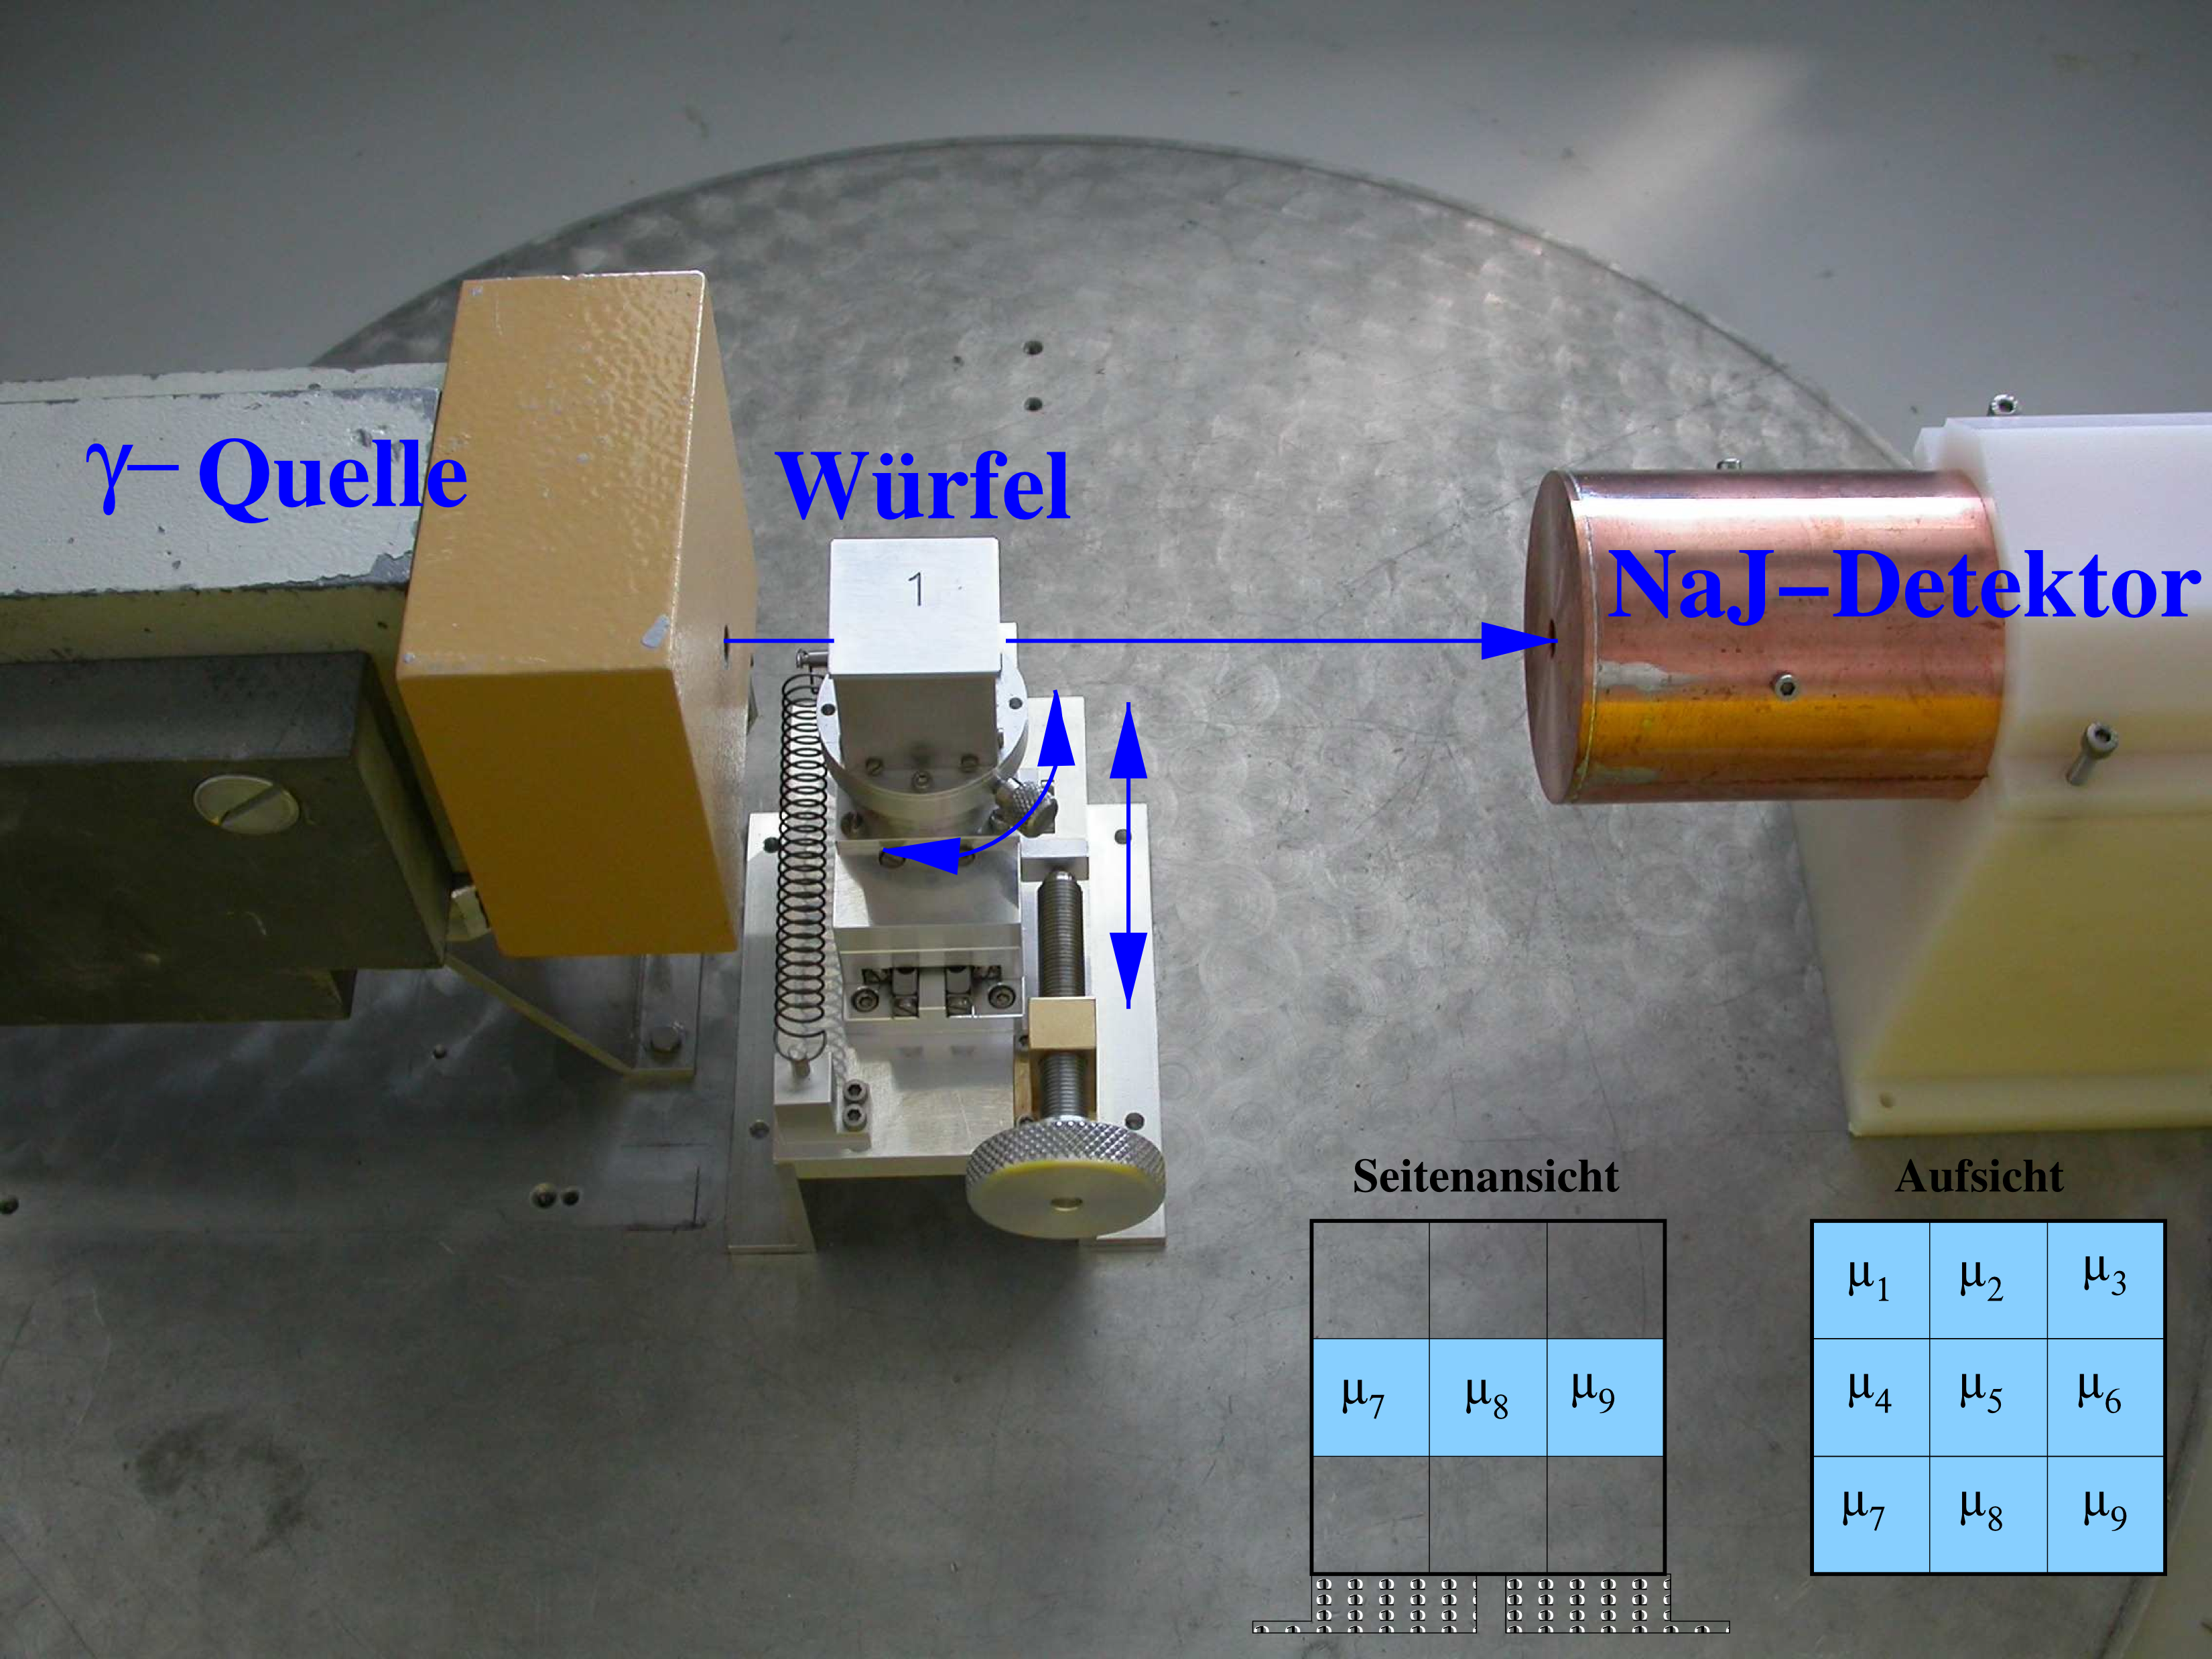
\includegraphics[width=\textwidth]{graphics/auf.png}
	\caption{Versuchsaufbau. \cite{Anleitung}}
	\label{fig:auf}	
\end{figure}
\subsection{Tomographische Vermessung}
Zuerst werden Referenzmessungen durchgeführt. Es werden ein leerer Aluminiumwürfel und 2 unbekannte massive Würfel aus den verschiedenen Projektionsrichtungen erst von außen auf ohre Größe vermessen und dann durchleuchtet.
Diese Werte dienen als Referenz für die Bestimmung von eventuellen Abweichungen.
Zwischen Strahlengang und Szintillationsdetektor wird der zusammengesetzte Würfel aus unterschiedlichen Richtungen durchleuchtet.
Die Intensität kann am Computer abgelesen werden. Dabei muss darauf geachtet, dass im Detektor wenigstens $1000$ Ereignisse gemessen werden, um eine, durch die Poissonverteilung der Zerfälle bedingte, Abweichung von weniger als $3\%$ zu gewährleisten.
